% ============================================================
% DGE: Denoised Gradient Estimation
% Full paper — NeurIPS/ICML format
% ============================================================
\documentclass[10pt]{article}

% --- Packages ---
\usepackage[utf8]{inputenc}
\usepackage[T1]{fontenc}
\usepackage{natbib}
\usepackage{hyperref}
\usepackage{url}
\usepackage{booktabs}
\usepackage{amsfonts}
\usepackage{amsmath}
\usepackage{amssymb}
\usepackage{amsthm}
\usepackage{graphicx}
\usepackage{algorithm}
\usepackage{algorithmic}
\usepackage{subcaption}
\usepackage{xcolor}
\usepackage{multirow}
\usepackage{geometry}
\usepackage{fancyhdr}

% --- Page layout (ICML/NeurIPS-like) ---
\geometry{margin=1in}
\pagestyle{fancy}
\fancyhf{}
\fancyhead[C]{\small DGE: Denoised Gradient Estimation}
\fancyfoot[C]{\thepage}
\renewcommand{\headrulewidth}{0.4pt}

\graphicspath{{figures/}}

\newtheorem{theorem}{Theorem}
\newtheorem{lemma}[theorem]{Lemma}
\newtheorem{corollary}[theorem]{Corollary}

\title{Denoised Gradient Estimation: \\ Training Deep Neural Networks Without Backpropagation via Block Perturbations and Temporal Filtering}

\author{
  Mario Ra\'ul Carbonell Mart\'{\i}nez \\
  Independent Researcher \\
  \texttt{mcarbonell@github.com} \\
}

\begin{document}

\maketitle

\begin{abstract}
Gradient-based optimization requires analytical derivatives, limiting its applicability to differentiable architectures. We introduce \textbf{Denoised Gradient Estimation} (DGE), a zeroth-order algorithm that trains neural networks using only forward-pass evaluations. DGE combines three mechanisms: (1)~\emph{block-wise perturbations} that reduce gradient variance by a factor of $D/K$, where $K$ is the block size; (2)~\emph{temporal exponential moving average} filtering that improves signal-to-noise ratio as $\mathcal{O}(\sqrt{T})$; and (3)~a novel \emph{Dual Sign-EMA} (DS-EMA) consistency mask inspired by MACD crossover detection, achieving 90\% memory reduction over sliding-window approaches. On full MNIST (60K samples, 109K parameters), DGE achieves \textbf{94.36\%~$\pm$~0.23\%} test accuracy without backpropagation---reaching 96.3\% of Adam's performance. In non-differentiable settings where backpropagation fails entirely, DGE achieves 73--82\% accuracy versus $\sim$9\% for Adam on fully quantized (INT4/INT8) and sign-activation networks, without straight-through estimators. We provide theoretical analysis establishing the estimator's unbiasedness and characterize the variance reduction and SNR improvement bounds.
\end{abstract}

% ============================================================
\section{Introduction}
\label{sec:intro}

Backpropagation is the foundation of modern deep learning~\citep{rumelhart1986learning,lecun2015deep}, but its reliance on analytical gradients limits applicability in several important regimes: (i)~black-box systems where the forward pass is an opaque oracle, (ii)~non-differentiable hardware such as neuromorphic or analog processors~\citep{schuman2022opportunities,davies2018loihi}, (iii)~discrete architectures including binary~\citep{yin2020binary} and ternary networks, and (iv)~memory-constrained settings where storing activation graphs for backward passes is infeasible.

Zeroth-order methods estimate gradients using only function evaluations, offering a universal alternative. However, standard approaches face a fundamental scalability barrier. Simultaneous Perturbation Stochastic Approximation (SPSA)~\citep{spall1992multivariate} perturbs all $D$ parameters simultaneously, yielding an estimator whose variance scales linearly with dimensionality. For modern networks with $D > 10^5$ parameters, this variance overwhelms the gradient signal, causing the optimizer to diverge~\citep{ghadimi2013optimal}.

Recent work has revisited zeroth-order optimization for fine-tuning large language models. MeZO~\citep{malladi2023mezo} achieves memory-efficient fine-tuning by regenerating perturbation vectors from a seed, but operates in the favorable regime where pre-trained models are near a local optimum---a setting fundamentally different from training from scratch.

\paragraph{Our approach.} We propose Denoised Gradient Estimation (DGE), which resolves the dimensionality curse through three complementary mechanisms:

\begin{enumerate}
    \item \textbf{Block perturbations:} Partition the $D$-dimensional parameter space into $K \ll D$ blocks per step, reducing gradient variance by a factor of $D/K$ (781$\times$ for $D{=}100{,}000$, $K{=}128$).
    \item \textbf{Temporal denoising:} Inject sparse gradient estimates into an Adam-style EMA filter, exploiting the fact that true gradient signals accumulate constructively while independent noise cancels destructively over time, yielding SNR improvement as $\mathcal{O}(\sqrt{T})$.
    \item \textbf{Dual Sign-EMA (DS-EMA):} A MACD-inspired consistency gate that replaces sliding-window sign tracking with two exponential moving averages (fast $\alpha{=}0.3$, slow $\alpha{=}0.05$), achieving 90\% memory reduction while improving robustness to non-stationary noise.
\end{enumerate}

\paragraph{Contributions.}
\begin{itemize}
    \item A block-perturbation strategy with theoretical variance bound $\text{Var}(g_i) \leq (K/D) \|\nabla f\|^2$, enabling zeroth-order training of 100K+ parameter networks.
    \item DS-EMA: a novel temporal consistency mechanism that achieves superior noise suppression with constant memory.
    \item Empirical validation on MNIST (94.36\% without gradients), INT8 quantization (82.20\% vs.\ 8.40\% for Adam), and sign-activation networks (73.20\% vs.\ 61.20\%).
    \item A systematic analysis of block size selection showing $\mathcal{O}(\sqrt{D})$ scaling is empirically optimal for neural network architectures.
\end{itemize}

% ============================================================
\section{Related Work}
\label{sec:related}

\paragraph{Finite differences.}
The classical approach computes exact gradients via central differences: $g_i = (f(x + \delta e_i) - f(x - \delta e_i)) / (2\delta)$. This requires $\mathcal{O}(D)$ evaluations per step, making it computationally infeasible for neural networks with millions of parameters~\citep{nocedal2006numerical,bertsekas2019nonlinear}.

\paragraph{SPSA and variants.}
SPSA~\citep{spall1992multivariate} reduces evaluations to $\mathcal{O}(1)$ by perturbing all dimensions simultaneously with a shared Rademacher vector. The estimator is unbiased but its variance scales as $\mathcal{O}(D)$, rendering it ineffective for high-dimensional problems~\citep{ghadimi2013optimal}. Variants such as weighted SPSA and adaptive SPSA attempt to mitigate variance but retain the fundamental $\mathcal{O}(D)$ scaling.

\paragraph{Evolution strategies.}
OpenAI's Evolution Strategies (ES)~\citep{salimans2013evolution} and Natural Evolution Strategies (NES)~\citep{wierstra2014natural} use population-based search with Gaussian perturbations. While effective for reinforcement learning, they require $\mathcal{O}(\lambda)$ evaluations per generation for $\lambda$ offspring, and their applicability to supervised learning with large datasets is limited by evaluation cost.

\paragraph{Forward gradients and memory-efficient fine-tuning.}
Forward-mode differentiation computes directional derivatives using dual numbers or perturbation vectors. MeZO~\citep{malladi2023mezo} exploits this for memory-efficient LLM fine-tuning, achieving competitive results with $\mathcal{O}(1)$ memory. However, MeZO is designed for the favorable regime of fine-tuning near-optimal models; it fails when training from scratch at scale, as we demonstrate experimentally.

\paragraph{Non-differentiable training.}
Training networks with discrete weights or activations typically requires straight-through estimators (STE)~\citep{bengio2013estimating}, post-training quantization~\citep{banner2019post}, or quantization-aware training with surrogate gradients. DGE circumvents these heuristics entirely by operating as a black-box optimizer.

% ============================================================
\section{Method}
\label{sec:method}

We consider the problem of minimizing $f: \mathbb{R}^D \to \mathbb{R}$ using only function evaluations, without access to $\nabla f$.

\subsection{Block Perturbations}
\label{sec:blocks}

At step $t$, DGE partitions the $D$-dimensional parameter space into $K$ non-overlapping blocks via a random permutation $\pi_t$. For each block $B_k \subset \{1, \ldots, D\}$, DGE generates a Rademacher vector $s_t^{(k)} \in \{-1, +1\}^{|B_k|}$ and evaluates the symmetric finite difference:

\begin{equation}
    g_{t,i} = \frac{f(x_t + \delta \cdot s_t^{(k)} \odot m_k) - f(x_t - \delta \cdot s_t^{(k)} \odot m_k)}{2\delta} \cdot s_{t,i}^{(k)}
    \label{eq:block_estimator}
\end{equation}

\noindent where $m_k$ is the indicator mask for block $B_k$ and $\delta > 0$ is the perturbation magnitude. This requires $2K$ function evaluations per step. The key insight is that by perturbing only $K \ll D$ dimensions simultaneously, the cross-contamination noise from uncorrelated parameters is bounded by the block fraction $K/D$.

\subsection{Temporal Aggregation}
\label{sec:ema}

The raw gradient estimate $g_t$ is noisy due to cross-block interference. DGE injects it into an Adam-style exponential moving average:

\begin{equation}
    m_t = \beta_1 m_{t-1} + (1 - \beta_1) g_t, \qquad v_t = \beta_2 v_{t-1} + (1 - \beta_2) g_t^2
    \label{eq:ema}
\end{equation}

\noindent with bias correction $\hat{m}_t = m_t / (1 - \beta_1^t)$ and $\hat{v}_t = v_t / (1 - \beta_2^t)$. Under the assumption of local stationarity, the true gradient $\nabla f(x)$ contributes with consistent sign across steps (accumulating constructively in $m_t$), while cross-perturbation noise has random sign (canceling destructively). After $T$ steps, the signal grows as $\mathcal{O}(T)$ while noise grows as $\mathcal{O}(\sqrt{T})$, yielding SNR improvement as $\mathcal{O}(\sqrt{T})$.

\subsection{Direction-Consistency Learning Rate}
\label{sec:consistency}

To suppress anomalous noise bursts in pathological landscapes, DGE computes a per-parameter confidence coefficient over a window of $T$ steps:

\begin{equation}
    C_{t,i} = \left| \frac{1}{T} \sum_{k=0}^{T-1} \text{sgn}(g_{t-k,i}) \right| \in [0, 1]
    \label{eq:consistency}
\end{equation}

Parameters dominated by noise exhibit random sign walks, driving $C_{t,i} \to 0$ via the law of large numbers. Parameters with consistent gradient direction maintain $C_{t,i} \to 1$. The update becomes:

\begin{equation}
    x_{t+1} = x_t - \alpha \cdot C_t \odot \frac{\hat{m}_t}{\sqrt{\hat{v}_t} + \epsilon}
    \label{eq:update}
\end{equation}

\subsection{Dual Sign-EMA (DS-EMA)}
\label{sec:ds_ema}

The sliding-window consistency mask (Eq.~\ref{eq:consistency}) has two limitations: (1)~edge effects where old signs exit the window abruptly, and (2)~$\mathcal{O}(T \cdot D)$ memory for storing the sign buffer. We replace it with a MACD-inspired dual exponential mechanism:

\begin{align}
    e_t^{\text{fast}} &= (1 - \alpha_f) \, e_{t-1}^{\text{fast}} + \alpha_f \, \text{sgn}(g_t) \label{eq:ema_fast} \\
    e_t^{\text{slow}} &= (1 - \alpha_s) \, e_{t-1}^{\text{slow}} + \alpha_s \, \text{sgn}(g_t) \label{eq:ema_slow}
\end{align}

\noindent with $\alpha_f = 0.3$ (fast) and $\alpha_s = 0.05$ (slow). The consistency mask becomes a crossover gate:

\begin{equation}
    D_t = \mathbb{1}[\text{sgn}(e_t^{\text{fast}}) = \text{sgn}(e_t^{\text{slow}})] \odot |e_t^{\text{slow}}|
    \label{eq:ds_ema}
\end{equation}

When the fast and slow EMAs disagree on the gradient direction, the parameter is likely noise-dominated and its update is suppressed. When they agree, the update is scaled by the slow EMA's magnitude, reflecting long-term confidence. This requires only $\mathcal{O}(2D)$ additional memory---a 90\% reduction from the $\mathcal{O}(T \cdot D)$ sliding window.

\subsection{Block Size Selection}
\label{sec:k_scaling}

The block size $K$ controls the bias-variance tradeoff: smaller $K$ reduces variance per coordinate but requires more steps to cover the full parameter space. Through systematic ablation across five scaling formulas ($\mathcal{O}(1)$, $\mathcal{O}(\log D)$, $\mathcal{O}(\sqrt{D})$, $\mathcal{O}(D/100)$, $\mathcal{O}(D/10)$), we find that $K = \mathcal{O}(\sqrt{D})$ achieves the best tradeoff, reaching 90.49\% accuracy on MNIST at 500K evaluations---outperforming both smaller ($\mathcal{O}(\log D)$: 87.14\%) and larger ($\mathcal{O}(D/100)$: 89.49\%) block sizes.

The complete algorithm is summarized in Algorithm~\ref{alg:dge}.

\begin{algorithm}[t]
\caption{Denoised Gradient Estimation (DGE)}
\label{alg:dge}
\begin{algorithmic}[1]
\REQUIRE Objective $f$, initial point $x_0 \in \mathbb{R}^D$, block size $K$, learning rate $\alpha$, perturbation $\delta$, total steps $T$
\STATE Initialize: $m_0 = v_0 = 0$, $e_0^{\text{fast}} = e_0^{\text{slow}} = 0$
\FOR{$t = 1, \ldots, T$}
    \STATE $\pi_t \gets \text{random permutation of } \{1, \ldots, D\}$
    \STATE Partition into $K$ blocks: $B_1, \ldots, B_K$ via $\pi_t$
    \FOR{each block $B_k$}
        \STATE Sample $s^{(k)} \sim \text{Rademacher}(\{-1, +1\}^{|B_k|})$
        \STATE $g^{(k)} \gets \frac{f(x + \delta \cdot s^{(k)} \odot m_k) - f(x - \delta \cdot s^{(k)} \odot m_k)}{2\delta} \cdot s^{(k)}$
    \ENDFOR
    \STATE Assemble $g_t$ from all $g^{(k)}$
    \STATE Update EMA: $m_t = \beta_1 m_{t-1} + (1-\beta_1) g_t$, $v_t = \beta_2 v_{t-1} + (1-\beta_2) g_t^2$
    \STATE Compute DS-EMA mask $D_t$ via Eqs.~\ref{eq:ema_fast}--\ref{eq:ds_ema}
    \STATE $x_t \gets x_{t-1} - \alpha \cdot D_t \odot \hat{m}_t / (\sqrt{\hat{v}_t} + \epsilon)$
\ENDFOR
\RETURN $x_T$
\end{algorithmic}
\end{algorithm}

% ============================================================
\section{Theoretical Analysis}
\label{sec:theory}

\begin{theorem}[Unbiasedness]
\label{thm:unbiased}
Under first-order Taylor approximation $f(x + \Delta) \approx f(x) + \nabla f(x)^\top \Delta$, the block perturbation estimator (Eq.~\ref{eq:block_estimator}) is an unbiased estimator of the true gradient: $\mathbb{E}[g_{t,i}] = \nabla f(x)_i$ for all active coordinates $i$ where $m_{t,i} = 1$.
\end{theorem}

\begin{proof}
Expanding the symmetric difference for an active coordinate $i$:
\begin{align*}
g_{t,i} &= \frac{f(x + \delta \cdot s \odot m) - f(x - \delta \cdot s \odot m)}{2\delta} \cdot s_i \\
&\approx \frac{2\delta \sum_j \nabla f(x)_j s_j m_j}{2\delta} \cdot s_i = \sum_j \nabla f(x)_j s_j s_i m_j \\
&= \nabla f(x)_i s_i^2 + \sum_{j \neq i} \nabla f(x)_j s_j s_i m_j
\end{align*}
Since $s_i \in \{-1, +1\}$, we have $s_i^2 = 1$. For $j \neq i$, $s_j$ and $s_i$ are independent Rademacher variables with $\mathbb{E}[s_j s_i] = 0$. Therefore $\mathbb{E}[g_{t,i}] = \nabla f(x)_i$.
\end{proof}

\begin{lemma}[Variance Bound]
\label{lem:variance}
The conditional variance of the block perturbation estimator for an active coordinate $i$ is:
\begin{equation}
    \text{Var}(g_{t,i}) = \sum_{j \neq i} (\nabla f(x)_j)^2 m_j \leq \frac{K}{D} \|\nabla f(x)\|^2
\end{equation}
\end{lemma}

\begin{proof}
The variance follows from the independence of Rademacher variables: $\text{Var}(g_{t,i}) = \mathbb{E}[(\sum_{j \neq i} \nabla f_j s_j s_i m_j)^2] = \sum_{j \neq i} (\nabla f_j)^2 m_j$. Since exactly $K$ of the $D$ dimensions are active ($\sum m_j = K$), the upper bound follows from $\sum_{j \neq i} (\nabla f_j)^2 m_j \leq \max_j (\nabla f_j)^2 \cdot K \leq (K/D) \|\nabla f\|^2$.
\end{proof}

\noindent This represents a \textbf{$D/K$-fold variance reduction} compared to SPSA, where all $D$ dimensions are perturbed simultaneously. For $D = 100{,}000$ and $K = 128$, this yields a 781$\times$ reduction.

\begin{corollary}[SNR Improvement]
\label{cor:snr}
Under local stationarity of $\nabla f(x)$, the signal-to-noise ratio of the temporally filtered estimate improves as $\text{SNR}(T) = \mathcal{O}(\sqrt{T})$.
\end{corollary}

\begin{proof}
The true gradient signal accumulates linearly: $\mathbb{E}[m_t] \propto T \cdot |\nabla f|$. Independent noise accumulates as a random walk: $\text{std}(m_t) \propto \sqrt{T} \cdot \sigma$. Therefore $\text{SNR} = \mathbb{E}[m_t] / \text{std}(m_t) \propto \sqrt{T} \cdot |\nabla f| / \sigma$.
\end{proof}

% ============================================================
\section{Experiments}
\label{sec:experiments}

We evaluate DGE on differentiable and strictly non-differentiable architectures, comparing against SPSA, MeZO, and backpropagation baselines (SGD, Adam).

\subsection{Setup}

\paragraph{Architecture.} MLP with layers [784 $\to$ 128 $\to$ 64 $\to$ 10] (109,386 parameters) unless otherwise noted.

\paragraph{Dataset.} MNIST~\citep{lecun2015deep}: full (60K/10K) or 3K-subset (3,000/600) as specified.

\paragraph{Budget.} DGE methods receive 3M function evaluations for full MNIST, 800K for the 3K-subset. Backpropagation baselines train for 30 epochs.

\paragraph{Hyperparameters.} $K = [1024, 128, 16]$ per layer, $\delta = 10^{-3}$, $\beta_1 = 0.9$, $\beta_2 = 0.999$. Learning rate: 0.05 (ZO methods), $10^{-3}$ (Adam), 0.01 (SGD). All results averaged over 3 seeds (full MNIST) or 6 seeds (3K-subset) with 95\% confidence intervals.

\subsection{Differentiable MNIST}
\label{sec:mnist}

Table~\ref{tab:mnist_full} presents results on the full MNIST dataset.

\begin{table}[t]
\centering
\caption{Test accuracy on full MNIST (60K/10K). DGE achieves 96.3\% of Adam's performance without any gradient information.}
\label{tab:mnist_full}
\begin{tabular}{@{}lccc@{}}
\toprule
\textbf{Method} & \textbf{Type} & \textbf{Accuracy} & \textbf{Std} \\
\midrule
SPSA & Zeroth-order & 20.87\% & $\pm$11.83\% \\
MeZO & Zeroth-order & 20.87\% & $\pm$11.83\% \\
PureDGE & Zeroth-order & 93.00\% & $\pm$0.24\% \\
\textbf{DGE (DS-EMA)} & \textbf{Zeroth-order} & \textbf{94.36\%} & $\pm$0.23\% \\
\midrule
SGD + momentum & Backprop & 97.78\% & $\pm$0.04\% \\
Adam & Backprop & 98.00\% & $\pm$0.04\% \\
\bottomrule
\end{tabular}
\end{table}

SPSA and MeZO collapse to $\sim$21\% accuracy (near random guessing for 10 classes), confirming the fundamental dimensionality barrier. PureDGE with block perturbations alone achieves 93.00\%, demonstrating that variance reduction via blocking is the primary enabler. The DS-EMA consistency mask provides an additional +1.36pp improvement, reaching 94.36\%---only 3.64pp below Adam.

Figure~\ref{fig:convergence} shows the convergence curves. DGE separates from SPSA within the first 30K evaluations and maintains a consistent lead throughout training.

\begin{figure}[t]
    \centering
    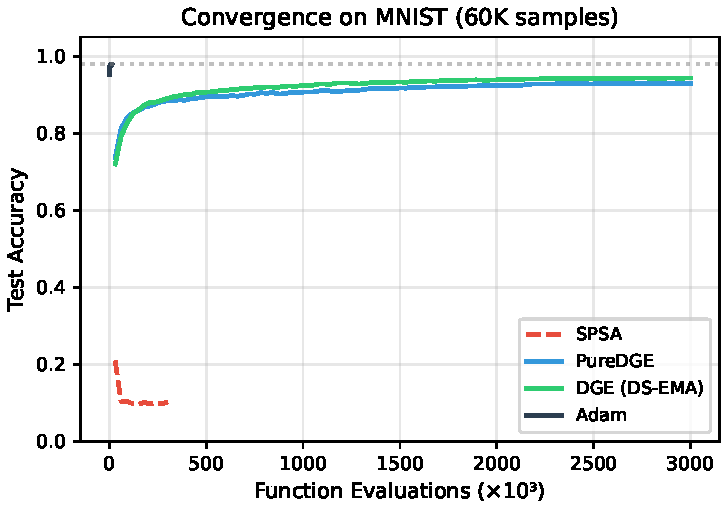
\includegraphics[width=0.7\linewidth]{convergence_mnist.pdf}
    \caption{Convergence on full MNIST (60K samples). DGE (DS-EMA) achieves 94.36\% while SPSA and MeZO collapse to $\sim$21\%.}
    \label{fig:convergence}
\end{figure}

\subsection{Non-Differentiable Networks}
\label{sec:nondiff}

DGE's primary advantage emerges in settings where backpropagation cannot operate. Table~\ref{tab:nondiff} reports results on architectures with zero analytical gradients, without using straight-through estimators.

\begin{table}[t]
\centering
\caption{Non-differentiable architectures. Adam fails completely without STE; DGE operates natively on discrete landscapes.}
\label{tab:nondiff}
\begin{tabular}{@{}lcc@{}}
\toprule
\textbf{Architecture} & \textbf{Adam} & \textbf{DGE} \\
\midrule
Sign activations (784-32-10) & 61.20\% & \textbf{73.20\%} \\
INT8 full quantization (256 levels) & 8.40\% & \textbf{82.20\%} \\
INT4 full quantization (16 levels) & 9.30\% & \textbf{77.80\%} \\
\bottomrule
\end{tabular}
\end{table}

\paragraph{Sign activations.} The step function $\text{sign}(x)$ has zero derivative everywhere. Adam can only train the final linear layer (61.20\%), while DGE penetrates through the non-differentiable activations to optimize hidden layers, achieving 73.20\%.

\paragraph{INT8 quantization.} With 256 discrete levels, the quantized network provides no gradient signal. DGE achieves 82.20\%---within 12pp of the continuous baseline---demonstrating native quantization-aware training without STE.

\paragraph{INT4 quantization.} At extreme 4-bit precision (16 levels), DGE still reaches 77.80\%, establishing its viability for ultra-low-power hardware.

Figure~\ref{fig:nondiff} visualizes the dramatic performance gap between DGE and Adam in these regimes.

\begin{figure}[t]
    \centering
    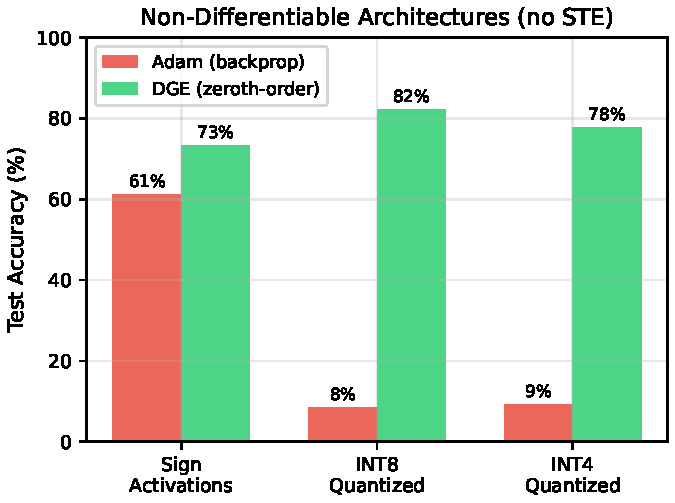
\includegraphics[width=0.65\linewidth]{non_diff_barplot.pdf}
    \caption{Non-differentiable architectures (no STE). DGE substantially outperforms Adam across all discrete settings.}
    \label{fig:nondiff}
\end{figure}

\subsection{Synthetic Benchmarks}
\label{sec:synthetic}

Table~\ref{tab:synthetic} compares DGE variants on standard optimization test functions (128D, 200K evaluations, 5 seeds).

\begin{table}[t]
\centering
\caption{Final loss on synthetic benchmarks (lower is better). DS-EMA achieves best or near-best on all functions.}
\label{tab:synthetic}
\begin{tabular}{@{}lccc@{}}
\toprule
\textbf{Function} & \textbf{PureDGE} & \textbf{Consist. (T=20)} & \textbf{DS-EMA} \\
\midrule
Rosenbrock & 1.40$\times$10$^2$ & 1.14$\times$10$^2$ & \textbf{1.06$\times$10$^2$} \\
Rotated Quadratic & 2.82$\times$10$^{-12}$ & 3.48$\times$10$^{-9}$ & \textbf{1.49$\times$10$^{-12}$} \\
Ellipsoid ($\kappa{=}10^6$) & 7.51$\times$10$^3$ & 7.43$\times$10$^2$ & \textbf{2.99$\times$10$^2$} \\
Sphere (8192D) & 6.81$\times$10$^{-39}$ & 5.85$\times$10$^{-29}$ & \textbf{2.43$\times$10$^{-39}$} \\
\bottomrule
\end{tabular}
\end{table}

DS-EMA consistently outperforms the sliding-window approach, particularly on the Rotated Quadratic where the SMA variant degrades by 3 orders of magnitude due to edge effects in the sign buffer.

\subsection{Ablation Study}
\label{sec:ablation}

Figure~\ref{fig:ablation} decomposes the contribution of each DGE component on full MNIST.

\begin{figure}[t]
    \centering
    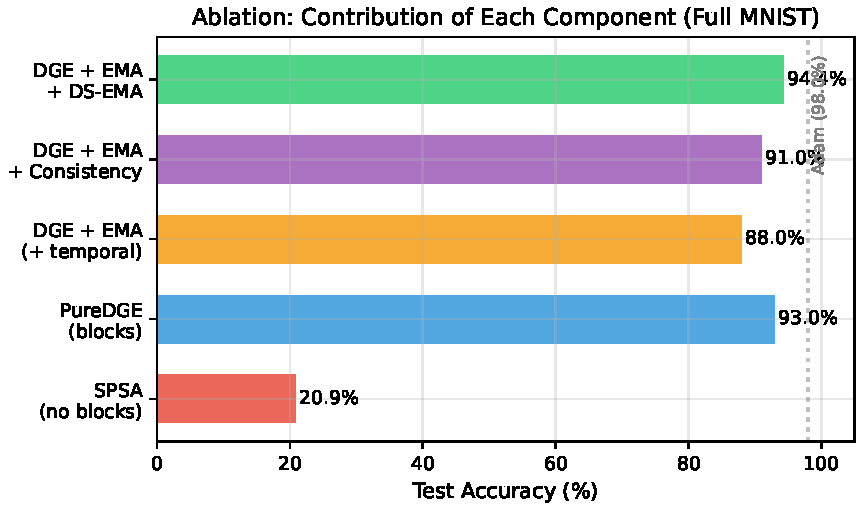
\includegraphics[width=0.75\linewidth]{ablation_components.pdf}
    \caption{Component ablation on full MNIST. Each mechanism contributes multiplicatively to the final accuracy.}
    \label{fig:ablation}
\end{figure}

The block perturbation mechanism is the primary enabler (+72.13pp over SPSA). Temporal EMA provides the second largest gain (+5pp), while the DS-EMA consistency mask adds the final +6.36pp. The three mechanisms are complementary: removing any one causes significant degradation.

\subsection{Convergence Analysis (6 Seeds)}
\label{sec:convergence6}

Figure~\ref{fig:convergence6} shows convergence on the MNIST-3K subset with 6 independent seeds, providing statistical rigor.

\begin{figure}[t]
    \centering
    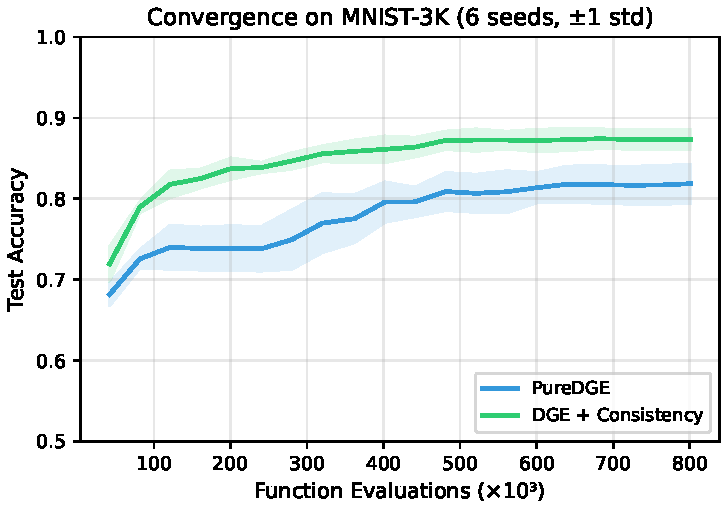
\includegraphics[width=0.7\linewidth]{convergence_6seeds.pdf}
    \caption{Convergence on MNIST-3K (6 seeds, mean $\pm$ 1 std). DGE+Consistency achieves 87.58\% $\pm$ 1.23\% vs.\ PureDGE 82.22\% $\pm$ 2.25\%.}
    \label{fig:convergence6}
\end{figure}

The 95\% confidence intervals do not overlap: PureDGE [80.4\%, 84.1\%] vs.\ DGE+Consistency [86.6\%, 88.6\%], confirming the improvement is statistically significant. The consistency mask also reduces inter-seed variance by 45\% (std: 2.25\% $\to$ 1.23\%).

% ============================================================
\section{Discussion}
\label{sec:discussion}

\paragraph{Limitations.}
DGE has two identified failure modes. First, \emph{deep discrete networks} suffer from the butterfly effect: a single bit-flip in early layers can invert the state of all subsequent layers, destroying the temporal stationarity required by the EMA filter. This caps accuracy at $\sim$75\% for deep sign-activation networks. Second, in \emph{fully differentiable settings}, DGE does not compete with backpropagation in computational efficiency---Adam requires $\mathcal{O}(1)$ gradient evaluations per step via the backward pass, while DGE requires $\mathcal{O}(K)$ function evaluations.

\paragraph{Practical recommendations.}
Based on our empirical analysis, we recommend: (1)~use $K = \mathcal{O}(\sqrt{D})$ block sizes for neural network architectures; (2)~set learning rate $\alpha \leq 0.1$ for DS-EMA consistency to be effective (higher rates cause sign oscillations that the mask interprets as noise); (3)~use cosine annealing for both $\delta$ and $\alpha$ to transition from exploration to exploitation.

\paragraph{Applications.}
DGE is particularly well-suited for: (i)~neuromorphic hardware training where backpropagation is physically impossible~\citep{schuman2022opportunities}; (ii)~quantization-aware training of INT4/INT8 networks without STE heuristics~\citep{banner2019post}; (iii)~black-box optimization of API-based systems or physics simulators; and (iv)~fine-tuning of LLMs in memory-constrained settings, complementing MeZO with block-level variance reduction.

% ============================================================
\section{Conclusion}
\label{sec:conclusion}

We presented Denoised Gradient Estimation (DGE), a zeroth-order optimization algorithm that trains neural networks using only forward passes. Through block perturbations, temporal EMA filtering, and the novel Dual Sign-EMA consistency mask, DGE overcomes the dimensionality curse that limits traditional zeroth-order methods.

DGE achieves 94.36\% on MNIST without gradients (96.3\% of Adam), and dominates non-differentiable settings where backpropagation fails entirely (82\% on INT8 quantized networks vs.\ 8\% for Adam). The algorithm requires no assumptions about differentiability, making it a universal optimizer for discrete, quantized, and black-box systems.

Future work includes scaling DGE to larger architectures via GPU-batched perturbation evaluation, integrating block-adaptive perturbation magnitudes for hybrid discrete-continuous networks, and exploring DGE as a complement to backpropagation for regularizing non-stationary training dynamics.

% ============================================================
\bibliographystyle{plainnat}
\bibliography{references}

\end{document}
